\chapter{Geschichtliche Übersicht}
\label{ch:Geschichtlich}

In der Geschichte von Hypertext sind viele verschiedene Konzepte und Systeme entstanden. In diesem Kapitel werden für einen Überblick einige davon vorgestellt. Das Konzept hinter Hypertext kann auf einen Artikel aus dem Jahr 1945 zurückgeführt werden.

\begin{quote}
	\glqq Consider a future device for individual use, which is a sort of mechanized private file and library. It needs a name, and to coin one at random, memex will do. A memex is a device in which an individual stores all his books, records, and communications, and which is mechanized so that it may be consulted with exceeding speed and flexibility.\grqq{ }\cite[Section 6]{Bush1945}.
\end{quote}

Im Jahr 1945 wurde \glqq As we may think\grqq{ }von Vannevar Bush veröffentlicht. Mit dem Konzept \glqq Memex\grqq{ } erdachte Vannevar Bush eine Maschine für die individuellen Verwendung - eine private, mechanisierte Bibliothek. Die \ref{fig:memex} zeigt eine Illustration aus dem Life Magazine 1945. Wenn der Nutzer ein bestimmtes Buch aufrufen möchte, könne er einen Code in das Keyboard eintippen und die Titelseite erscheint als Projektion \cite[S.121]{Life1945} \cite[Section 6]{Bush1945}. In in diesem Konzept könne der Nutzer einen sogenannten \glqq main trail\grqq{ }aus Dokumenten erstellen. Dieser Trail solle eine Kombination aus Dokumenten sein, die aus der Perspektive des Nutzers von Interesse ist. Mit sogenannten \glqq side tails\grqq{ }könne der Nutzer ein Main Trail mit anderen Dokumenten \glqq verlinkt\grqq{ }\cite[Section 7]{Bush1945}. Diese Trails könnten als erstes Konzept von Hyperlinks verstanden werden. Zwei Jahrzehnte nach der Veröffentlichung von \glqq As we may think\grqq{ }, in der 1960er Jahren, wurde der erst der Begriff Hypertext von Ted Nelson geprägt. 

\begin{figure}[!ht]
	\centering
	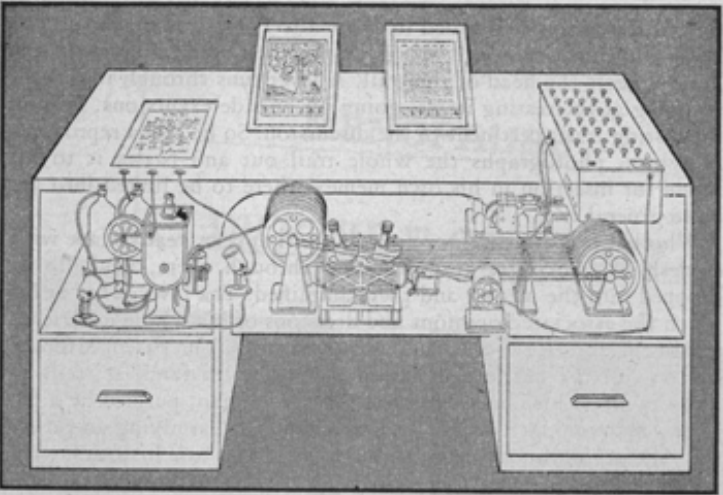
\includegraphics[width=0.6\textwidth]{image/memex}
	\caption{\glqq Memex in the form of a desk would instantly bring files and material on any subject to the operator's fingertips. [...] At left is a mechanism which automatically photographs longhead notes, pictures and letters, then files them in the desk for future reference\grqq{ } \cite[S.123]{Life1945}}
	\label{fig:memex}
\end{figure}

\begin{quote}
	\glqq Let me introduce the word hypertext to mean a body of written or pictorial material interconnected in such a complex way that it could not conveniently be presented or represented on paper. It may contain summaries, or maps of its contents and theier interrelations; it may contain annotations, additions and footnotes from scholars who have examined it. [...]\grqq{ }\cite{Nelson1965}
\end{quote}

Nach Ted Nelson habe ein System auf Papier gravierende Einschränkungen beim Organisieren oder Präsentieren von Ideen. Ein Buch würde nie perfekt zu einem Leser passen. Der eine Leser sei gelangweilt, während ein anderer von den gleichen Seiten verwirrt werde. \glqq Ein solches System könne das Potenzial haben, das Gefühl der Freiheit, die Motivation und das intellektuelle Verständnis des Lesenden zu vergrößern\grqq{ }\cite{Nelson1965}. 

\begin{section}{NLS und AUGMENT}
\label{sec:nls}

Im gleichen Jahrzehnt erschien Doug Engelbarts \glqq Augmenting Human Intellect: A Conceptual Framework\grqq{ }. 

\begin{quote}
\glqq By augmenting human intellect we mean increasing the capability of a man to approach a complex problem situation [...].\grqq{ }\cite[S. 1]{Engelbart1962}
\end{quote}

Engelbart schrieb in \glqq Augmenting Human Intellect: A Conceptual Framework\grqq{ } von dem \glqq digital computer as a tool for the personal use of an individual. Here there is not only promise of great flexibility in the composing and rearranging of text [...]\grqq{ }\cite[S. 17]{Engelbart1962}. Während seiner Arbeit am Augmentation Research Center am Stanford Research Institute (SRI-ARC) wurde unter anderem das \glqq NLS\grqq{ }(the oN-Line System) entwickelt. Wobei \glqq on-line\grqq{ }in den 60er Jahren nicht die gleiche Bedeutung gehabt haben dürfte als Heute. Vorgestellt wurde das NLS auf der Fall Joint Computer Conference in San Francisco 1968. Diese Präsentation wird oft \glqq mother of all demos\grqq{ }genannt. Neben dem NLS wurden auch die interaktive Textverarbeitung, die Computermaus und die Organisation von Windows auf dem Bildschirm (Siehe \ref{fig:mother}). Das NLS würde präsentiert als \glqq ein mächtiges Tool für die Arbeit eines Individuums, wenn er studiert, plant, designt, debuggt oder dokumentieren.\grqq{ }\cite{MotherOfDemo1968}. Es gäbe Möglichkeiten für das kollaborative Arbeiten, es gäbe gemeinsame Dokumente und man könne Nachrichten an Dokumente heften \cite{MotherOfDemo1968}. 

\begin{figure}[!ht]
	\centering
	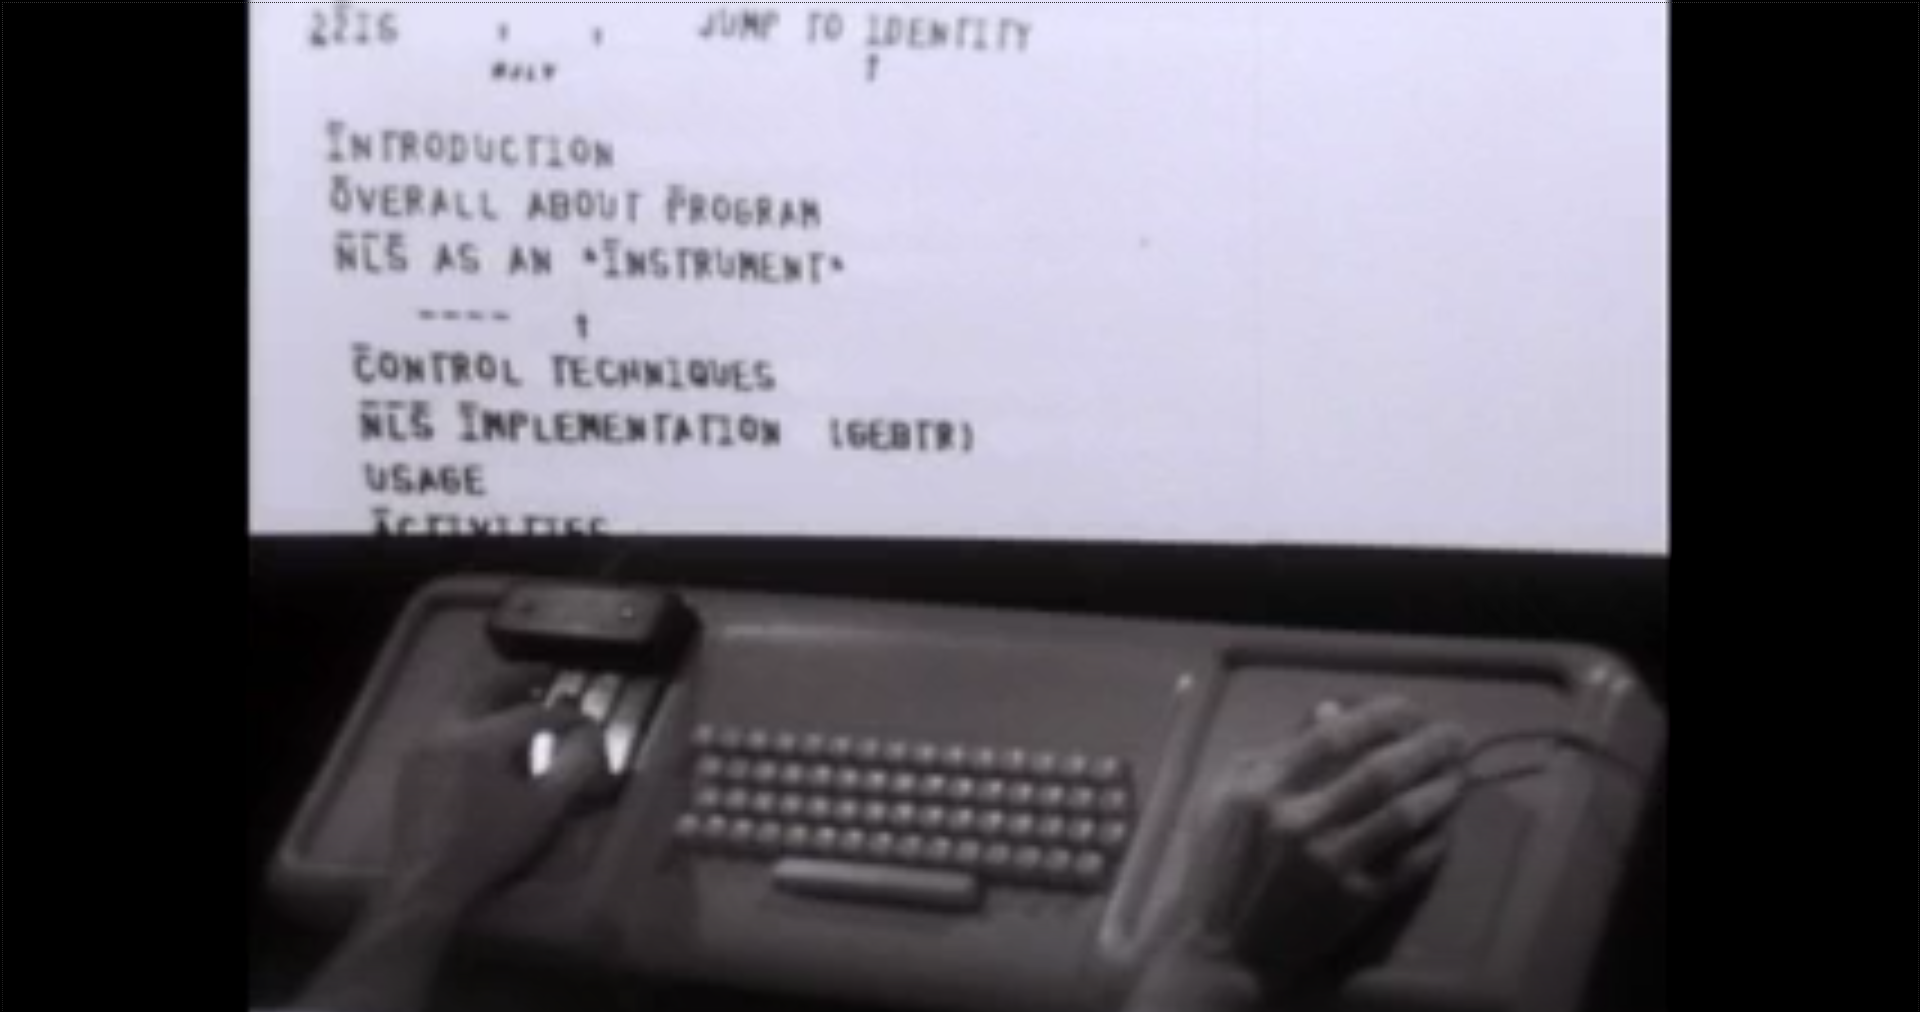
\includegraphics[width=0.8\textwidth]{image/mother}
	\caption{Doug Engelbart präsentiert auf der Fall Joint Computer Conference in San Francisco die Forschung vom Stanford Research Institute \cite{MotherOfDemo1968}.}
	\label{fig:mother}
\end{figure}

Gezeigt wurden aber auch die Hypertext Funktionalitäten, Dokumente seien verknüpft mit Links und der Nutzer könne entscheiden welchen \glqq Branch\grqq{ }er betrete \cite{MotherOfDemo1968}. Verlinkungen konnten durch verschiedene Adressiermöglichkeiten realisiert werden. Jedes Dokument in NLS ist in \glqq Statements\grqq{ }unterteilt und diese Statements konnten auf verschiedene Weisen verlinkt werden \cite{Engelbart1984}. Jedes Statement hat eine \glqq structural statement number\grqq{ }, eine eindeutige ID, die sind nach der Position in einem Dokument richtet. Nach dem Verändern des Textes konnten so Links zu falschen Statements führen. Der \glqq statement identifiers\grqq{ }, als globale ID war unabhängig von der Position des Statements, diese ID blieb unverändert und \glqq Labels\grqq{ }die vom Nutzer definiert werden. Das Userinterface bot Kommandos zum Manipulieren der Oberfläche. Die interaktive Textbearbeitung unterstützte Funktionen wie Insert, delete, Move and Copy. Es konnten Outlines und eine Art Vorschau der ersten Zeilen von jedem Statement angezeigt werden. Die Verlinkungen und Bedienmöglichkeiten ermöglichten dem Nutzer ein \glqq herein und heraus zoomen \grqq{ }\cite{MotherOfDemo1968}. Die kommerziellen Rechte an dem System wurden 1978 an Tymshare abgegeben und NLS wurde zu AUGMENT umbenannt \cite{Engelbart1984}. Im Vergleich zum Konzept Memex hatte das Team um das NLS ähnliche Ziele. Die Arbeit des Individuums sollte optimiert werden. Die Memex als analoges Konzept und das NLS als digitale Lösung für ein Hypertext-System. Die Verknüpfungen der Dokumente in der Memex Maschine sind vergleichbar mit den verlinkten Statements im NLS, beide Verlinkungen wurden auch über IDs realisiert \cite{Engelbart1984}, \cite{Bush1945}. Nur die Navigation durch die Links unterschied sich bei beiden, statt Touch und Spracheingabe \cite{Bush1945} nutzte das Team rund um Doug Engelbart Maus und Tastatur \cite{MotherOfDemo1968}.

\end{section}

\begin{section}{Problem: Dangling edges}
\label{sec:dangling}

Allerdings wäre Vannevar Bush bei einer Realisierung der Memex wahrscheinlich auf das gleiche Problem gestoßen wie Doug Engelbart. Ein Hypertext ist vergleichbar mit einem Graphen aus Nodes und Edges. Ein Text könnte ein Node sein und eine Verlinkungen zwischen zwei Texten ist eine Edge zwischen zwei Nodes. Durch entfernen von Nodes können \glqq dangling edges\grqq{ }entstehen. Die \ref{fig:dangle} zeigt zum Beispiel durch das Entfernen des Textes $D$ zwei entstandenen Dangling Edges von $A$ und $E$. Bei NLS konnte durch das Bearbeiten der Dokumente oder Statements Dangling Edges entstehen. Dies könnte durch die verschiedenen Adressiermöglichkeiten zumindest eingedämmt werden \cite{Engelbart1984}.

\begin{figure}[!ht]
	\centering
	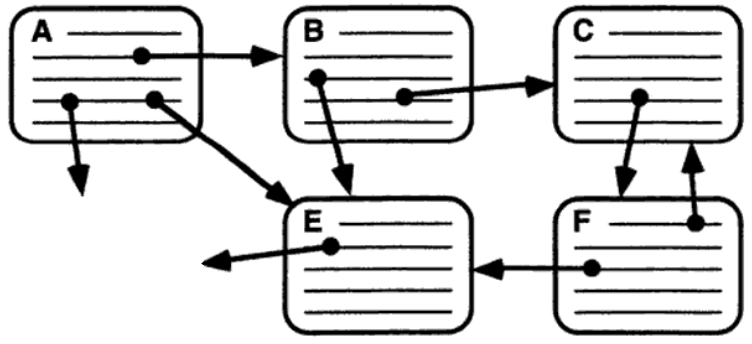
\includegraphics[width=0.8\textwidth]{image/dangle}
	\caption{Modifizierte Darstellung von Nielsen, zur Darstellung von zweier Dangling Edges \cite[S.1]{Nielsen1995}.}
	\label{fig:dangle}
\end{figure}

\end{section}

\begin{section}{HES}
\label{sec:hes}

Ebenfalls in dem 1960er Jahren wurde an der Brown Universität, im US-amerikanischen Bundesstaat Rhode Island, ein Hypertext-System Namens \glqq HES\grqq{ } (Hypertext Editing System) entwickelt. 1967 begannen Andries van Dam und Ted Nelson die Entwicklung an HES. Eigentlich sei der Zweck von HES gewesen, das Hypertext Konzept zu erforschen, später sei es von IBM aber auch an die NASA verkauft worden und zur Dokumentation der Apollo Missionen verwendet worden \cite{Dam1988}.

\begin{quote}
\glqq One of the most important things (Nelson) taught me was that this is a new medium and you really can’t be constrained to thinking about it in the old ways. Don‘t copy old, bad habits; think about new organizations, new ways of doing things, and take advantage of this new medium.\grqq{ }\cite{Dam1988}
\end{quote}

Texte konnten in HES in separate Sektionen unterteilt werden. Grundlegend gab es zwei verschiedene Verlinkungen in HES, \glqq Links\grqq{ }und \glqq Brachnes\grqq{ }. Branches wurden organisiert im Branch Menü oder waren im späteren Ausdruck als Fußnoten zu sehen. Links konnten optional vom Nutzer besucht werden. Beide waren im Text markiert mit einem Sternchen (*) und zeigten einen sogenannten Explainer als Vorschau an. Der Explainer eines Links tauchte in der Annotaion Area auf, der Branch Explainer wurde in-line beim Branch Sternchen angezeigt. Der Nutzer konnte Sektionen mit dem Lightpen auswählen und einem einzigartigem Label versehen. Dieses Label wurde dann in eine Label Tabelle eingetragen werden und konnten mit dem Befehl besucht werden und als Pointer in einem Text verwendet werden \cite{Dam1969}. Die Texte selbst waren sogenannte Instanzen und wurden unidirektional verlinkt. Die Bearbeitung selbst sei mehr eine Pointer Manipulation als Text Manipulation gewesen \cite[S. 890]{Dam1988}.

\begin{quote}
\glqq Instances are references, so that if you changed, for example, a piece of legal boilerplate that was referenced in multiple places, the change would show up in all the places that referenced it. \grqq{ }\cite{Dam1988}
\end{quote}

Dem Nutzer war die Möglichkeit gegeben, nach dem Drücken eines \glqq Function Keys\grqq{ }mit dem Lightpen einen Link zu berühren und so dem Link zu folgen \cite[S.23]{Dam1969}. Wie auch das NLS unterstützte die Textbearbeitung Funktionen wie Insert, Delete, Move and Copy \cite[S.10-14]{Dam1969}, \cite[S. 889]{Dam1988}. Beim entfernen vom Text entstanden keine Dangling Edges, wie in \ref{sec:dangling} beschrieben. Jeder Link oder Branch der auf die gelöschte Sektion zeigt wird ebenfalls gelöscht \cite[S.12]{Dam1969}.

\begin{figure}[!ht]
	\centering
	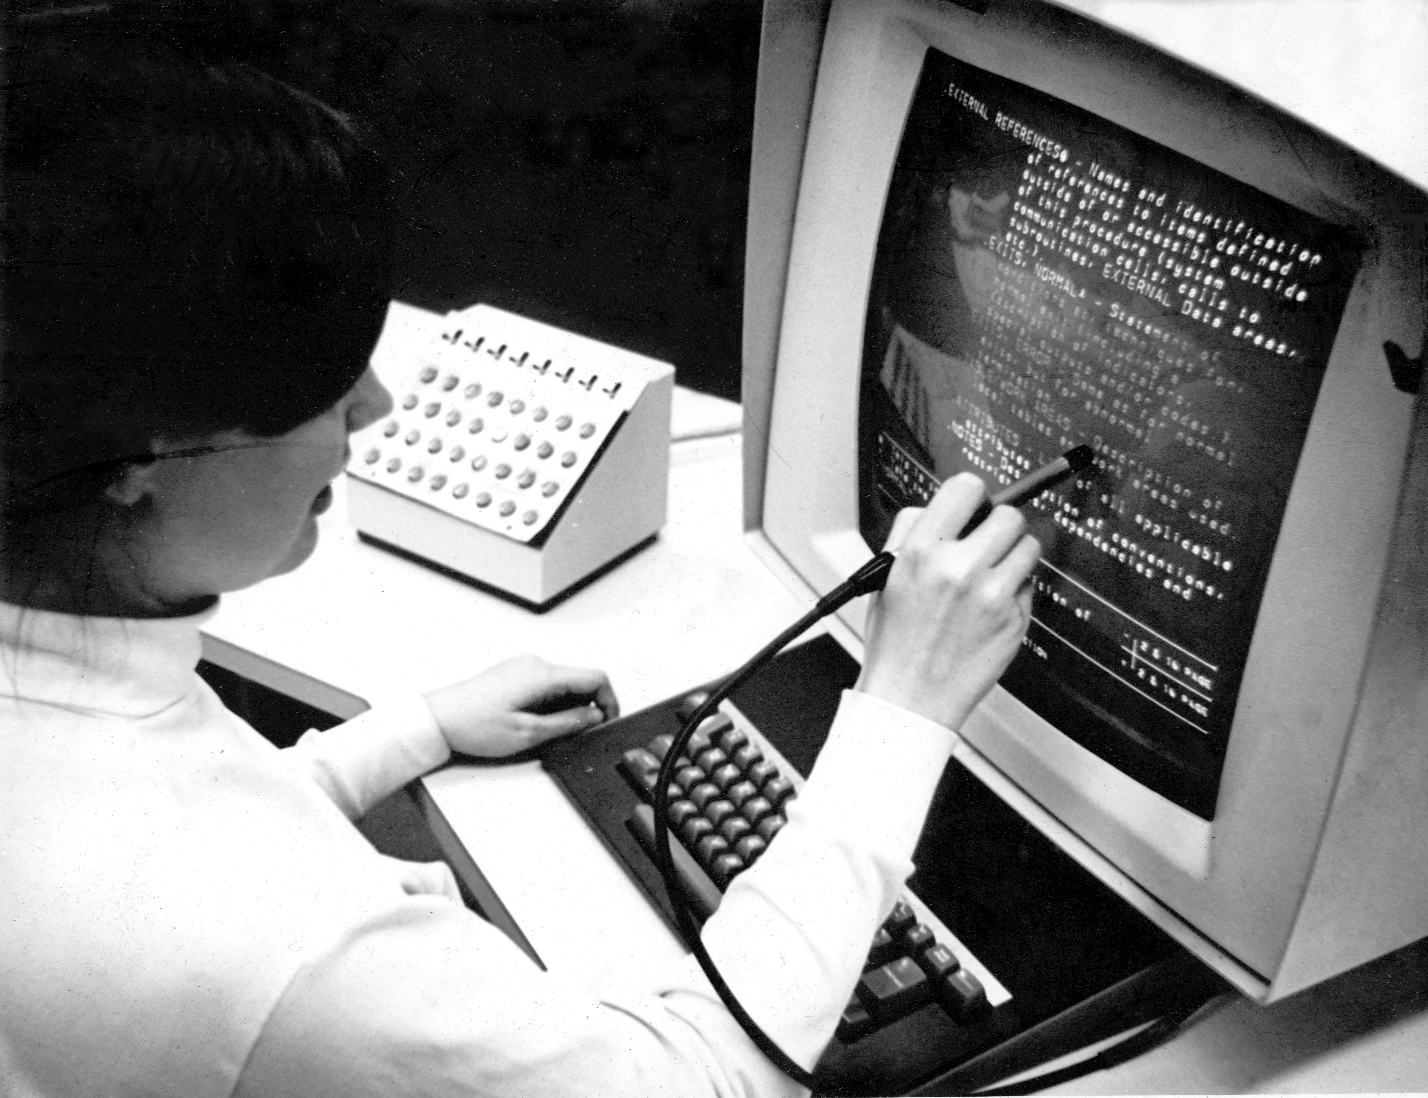
\includegraphics[width=0.8\textwidth]{image/hes}
	\caption{Foto einer von HES in der Brown Universität \cite{Lloyd1969}.}
	\label{fig:hes}
\end{figure}

\end{section}

\begin{section}{FRESS}
\label{sec:fress}
	
1968 startete van Dam zusammen mit seinen Stunden die Entwicklung von \glqq a File Retrieval and Editing System\grqq{ }(FRESS). Inspiriert von Doug Engelbart sollte FRESS die besten Ideen von NLS und HES vereinen \cite[S.887 und 890]{Dam1988}. FRESS sollte auch auf verbreiteten kommerziellen Systemen laufen. Van Dam zufolge sei FRESS das erste System gewesen, dass eine UNDO Funktion unterstützte. Jede Bearbeitung wurde in einener Schattenversion gespeichert und erlaubte so ein Autosave und ein UNDO \cite[S.891]{Dam1988}. Im Gegensatz zum Vorgänger unterstützte FRESS bidirektionale Links, so genannte \glqq Jumps\grqq{ }. Aber weiterhin gab es auch on-way Links, die sogenannten \glqq Tags\grqq{ }. Paul Delany und George P. Landow schrieben hierzu: \glqq FRESS had two types of links - indicated a connection to a single element such as an annotation, definition, or footnote. When the reader pointed to a tag with a light pen, the associated text appeared in another window on the screen for reference while the reader remained in the main document. Unlinke a tag, a jump - a bidirectional link - indicated a path to another document. By following a jump, the reader was transferred from one document to another, and up to seven windows could be used to display documents simultaneously. \grqq{ }\cite[S.68]{GeorgeLandow1995}. FRESS unterstütze so den Nutzer beim Navigieren durch die Links, außerdem konnte so der Autor, wie schon bei der Memex angedacht, eine Art Main Track oder Side Tracks erstellen. Im Text wurden die \glqq cross-reference markers\grqq{ }angezeigt, diese zeigten dem Nutzer alle Verlinkungen an und gaben dem Leser einen \glqq Backtrack\grqq{ }durch seine besuchten Links. Links waren in FRESS eigene Objekte und nicht mehr einfach Teile eines Textes. Es sei möglich gewesen Links zu typisieren oder zu labeln, indem man sie mit \glqq key words\grqq{ }versehe \cite[S.891]{Dam1988}. Das System wurde auf Grund des hohen Funktionsumfang nicht fertig gestellt, van Dam schrieb \glqq It was overkill, and we haven’t done it since, but it certainly was interesting.\grqq{ }\cite[S.891]{Dam1988}.

\end{section}

\begin{section}{Problem: Lost in Hyperspace}
\label{sec:lostInHyperspace}

Je komplexer und größer ein Hypertext Graph wird, desto einfacher kann man sich auf der viel zahl von Branches verlieren. So auch van Dam: \glqq We already started getting the notion that the richer the hypertext, the greater the navigational problem. \grqq{ }. Nach van Dam sei das \glqq come from\grqq{ } genauso wichtig wie das \glqq go to\grqq{ }\cite{Dam1988}.

\begin{quote}
\glqq [...] The real diagram was about the size of a large blueprint [...]. We had already come to the point where Ted, who designed it, was able to go through the hypertext pretty well, but some of the rest of us had difficulty following it-it was not exactly obvious where you were. This, of course, is the classical lost-inhyperspace problem [...]\grqq{ }\cite{Dam1988}
\end{quote}

FRESS nutzte beim Aufruf von Links Beispielsweise Windows und bidirektionale Links damit der Nutzer sich nicht im Hyperspace verloren geht. In der Memex wäre dieses Problem eventuell durch die zwei Anzeigen ein wenig entschärft worden, aber auch hier wäre man beim Navigieren durch die Dokumente irgendwann \glqq lost in hyperspace\grqq. Erst die bidirektionalen Links und Windows lösen dieses Problem und geben dem Nutzer die Möglichkeit seinen Weg zurück zugehen.

\end{section}

\begin{section}{}
\label{sec:lostInHyperspace}

\end{section}